\documentclass{article}

% Language setting
% Replace `english' with e.g. `spanish' to change the document language
\usepackage[english]{babel}

% Set page size and margins
% Replace `letterpaper' with`a4paper' for UK/EU standard size
\usepackage[letterpaper,top=2cm,bottom=2cm,left=3cm,right=3cm,marginparwidth=1.75cm]{geometry}

% Useful packages
\usepackage{amsmath}
\usepackage{graphicx}
\usepackage[colorlinks=true, allcolors=blue]{hyperref}
\usepackage{tabularx}
\usepackage{fvextra}

\title{Rapport d'avancement}
\author{Vital FOCHEUX}
\date{du 5 juin au 12 juin 2026}

\begin{document}
\maketitle

\section{Notes de la dernière réunion}

\begin{itemize}
    \item Qu'il faut faire des schémas pour comprendre où sont situés les différents filtres dans le système
    \item Faire un filtre passe-haut pour avoir plus de modularité
    \item Faire en sorte que les filtres puissent être utilisés indépendamment des contrôleurs pour pouvoir les utiliser ailleurs
    \item Faire une figure pour représenter l'intégral au cours du temps pour les anti-windup
    \item Bien définir les équations mathématiques pour les filtres et les anti-windup
\end{itemize}

\section{Depuis la dernière fois}

\subsection{Planning}

Avec Anna on s'est fixé un planning pour les prochaines semaines jusqu'à la fin du mois de juin, qui est le suivant :
\begin{itemize}
    \item du 8 au 12 juin : 
    \begin{itemize}
        \item Correction du modèle de drone $\rightarrow$ pour qu'il fonctionne avec une consigne plus cohérente (5 mètres) et qu'on observe des résultats différents entre avec/sans anti-windup
        \item Séparation filtres/contrôleurs
        \item Clarifier l'interface chips $\rightarrow$ montrer comment utiliser Filtre/Anti-windup en chips avec description bloc fonctionnel et documentation
        \item Plan détaillé du rapport de stage
    \end{itemize}
    \item du 15 au 19 juin :
    \begin{itemize}
        \item Rédaction du package contrôleur chips (diagramme bloc fonctionnel + chips) $\rightarrow$ tester (via BIP)
        \item Des plots et diagrammes (pour analyser les résultats)
        \item Mise en commun avec Julien (travaux futurs)
    \end{itemize}
    \item du 22 au 26 juin :
    \begin{itemize}
        \item Rédaction du rapport de stage
        \item Lien formel travaux Vital / Motif control
    \end{itemize}
\end{itemize}

\subsection{Filtres}

Je me suis rendu compte que les exemples que j'utilisais sur les filtres utilisaient un contrôleur PID, mais qu'il 
n'y avait pas de boucle de rétroaction.
J'ai sorti les filtres des contrôleurs pour les utiliser indépendamment comme ce qu'on aimerait pouvoir faire dans 
n'importe quel système.

\subsubsection{Passe-Bas et Passe-Haut}

Pour chacun de ces 2 filtres, je génère un ensemble de valeurs brut en utilisant cette équation :
$$y = \sin(1.2 * 2 * \pi * t) + 1.5 * \cos(0.8 * 2 * \pi * t) + 0.5 * \sin(2 * 2 * \pi * t)$$

Où t est la variable de temps allant de 0 à 150 secondes avec un pas de $\frac{1}{30}$ secondes.

Le but est de voir comment les filtres réagissent à différentes fréquences de signal.

Pour le filtre passe-bas, l'équation est la suivante :
$$\alpha = \tau / (\tau + dt)$$
$$y_n = \alpha * y_{n-1} + (1 - \alpha) * x_n$$

Où :
\begin{itemize}
    \item $\tau$ est la constante de temps du filtre, qui détermine la rapidité avec laquelle le filtre réagit aux changements de signal
    \item $dt$ est le pas de temps entre les échantillons
    \item $y_n$ est la sortie du filtre à l'instant n
    \item $y_{n-1}$ est la sortie du filtre à l'instant n-1
    \item $x_n$ est l'entrée du filtre à l'instant n
\end{itemize}

Pour le filtre passe-haut, l'équation est la suivante :
$$\alpha = \tau / (\tau + dt)$$
$$y_n = \alpha * (y_{n-1} + x_n - x_{n-1})$$

Où :
\begin{itemize}
    \item $\tau$ est la constante de temps du filtre, qui détermine la rapidité avec laquelle le filtre réagit aux changements de signal
    \item $dt$ est le pas de temps entre les échantillons
    \item $y_n$ est la sortie du filtre à l'instant n
    \item $y_{n-1}$ est la sortie du filtre à l'instant n-1
    \item $x_n$ est l'entrée du filtre à l'instant n
    \item $x_{n-1}$ est l'entrée du filtre à l'instant n-1
\end{itemize}

Pour les 2 filtres, j'ai choisi une constante de temps $\tau$ égale à $\frac{1}{(2 * \pi * 3.667)} \approx 0.043$ secondes et un pas de temps $dt$ de $\frac{1}{30}$ secondes.

On peut voir sur les schémas à quel niveau du système les filtres sont appliqués. (cf figures \ref{fig:schema_lowpass}, \ref{fig:schema_highpass} et \ref{fig:schema_highpass_lowpass})

Le filtre passe-bas laisse passer les basses fréquences et atténue les hautes fréquences, tandis que le filtre 
passe-haut fait l'inverse. En combinant les deux filtres, on peut créer un filtre passe-bande qui laisse passer 
une plage de fréquences spécifique.

Pour le filtre passe-bas (cf figure \ref{fig:lowpass}), on peut voir que les hautes fréquences sont atténuées, 
tandis que les basses fréquences sont préservées. Pour le filtre passe-haut (cf figure \ref{fig:highpass}), on 
peut voir que les basses fréquences sont atténuées, tandis que les hautes fréquences sont préservées. Enfin, pour 
le filtre passe-haut puis passe-bas (cf figure \ref{fig:highpass_lowpass}), on peut voir que les fréquences ne dépassent pas une certaine plage, ce qui correspond à un filtre passe-bande.



\begin{figure}
    \centering
    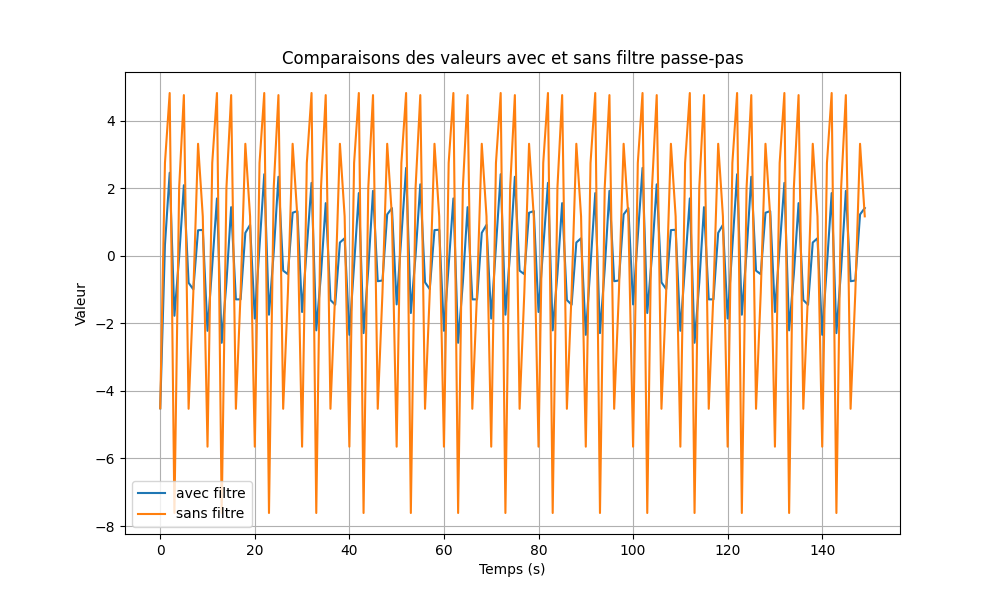
\includegraphics[width=\textwidth]{passe_bas.png}
    \caption{Résultat du filtre passe-bas sur les données}
    \label{fig:lowpass}
\end{figure}

\begin{figure}
    \centering
    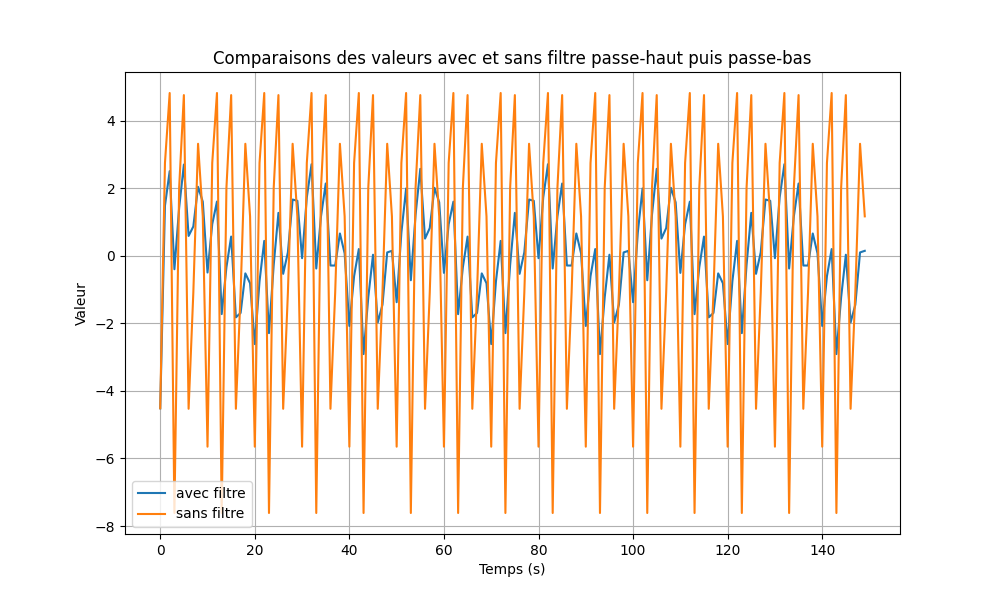
\includegraphics[width=\textwidth]{passe_haut_passe_bas.png}
    \caption{Résultat du filtre passe-haut puis passe-bas sur les données}
    \label{fig:highpass_lowpass}
\end{figure}

\begin{figure}
    \centering
    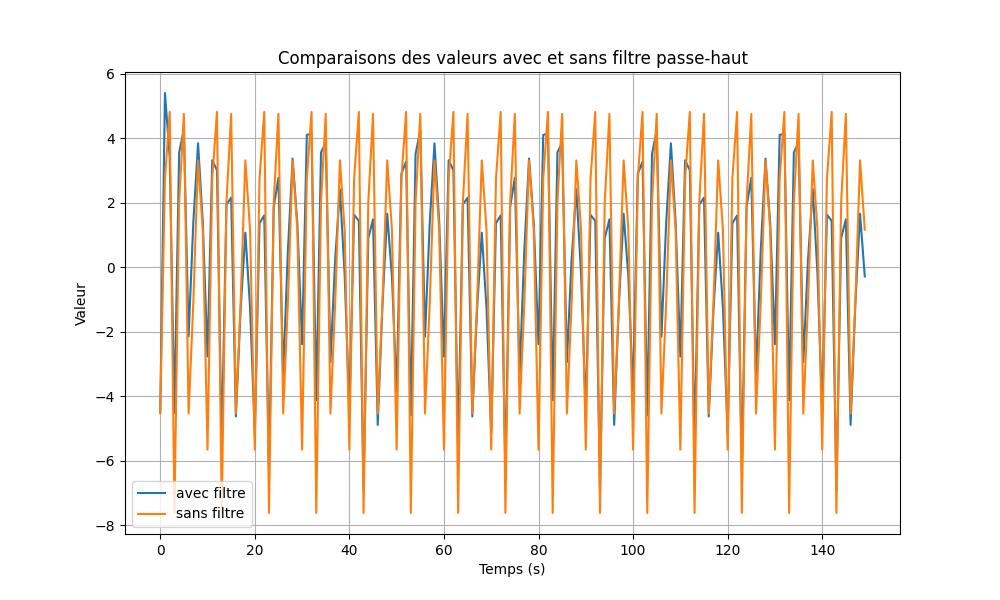
\includegraphics[width=\textwidth]{passe_haut.png}
    \caption{Résultat du filtre passe-haut sur les données}
    \label{fig:highpass}
\end{figure}

\begin{figure}
    \centering
    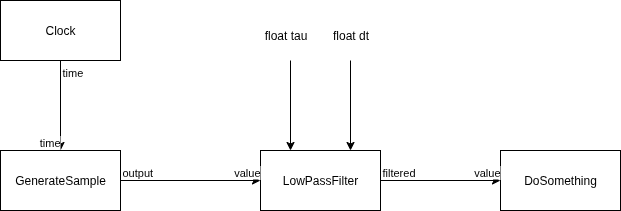
\includegraphics[width=\textwidth]{schema_lowpass.png}
    \caption{Schéma du filtre passe-bas}
    \label{fig:schema_lowpass}
\end{figure}

\begin{figure}
    \centering
    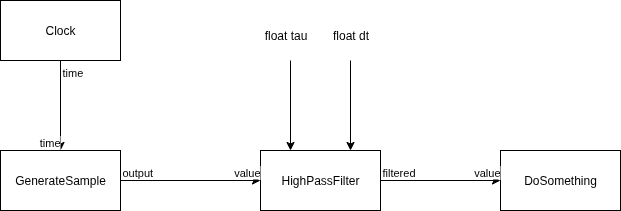
\includegraphics[width=\textwidth]{schema_highpass.png}
    \caption{Schéma du filtre passe-haut}
    \label{fig:schema_highpass}
\end{figure}

\begin{figure}
    \centering
    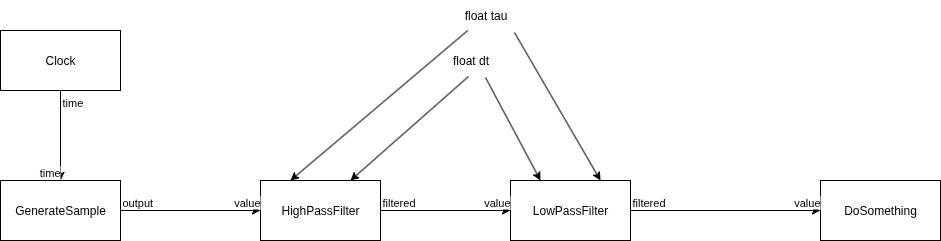
\includegraphics[width=\textwidth]{schema_highpass_lowpass.png}
    \caption{Schéma du filtre passe-haut puis passe-bas}
    \label{fig:schema_highpass_lowpass}
\end{figure}

\subsubsection{Médian}

Tout comme les exemples précédents, j'utilise une équation pour générer un ensemble de valeurs brut :
$$y = \sin(2 * \pi * freq * time)$$

où :
\begin{itemize}
    \item freq est la fréquence du signal, que j'ai choisie égale à 0.2 Hz
    \item time est la variable de temps allant de 0 à 200 secondes avec un pas de 0.05 secondes
\end{itemize}

J'ajoute ensuite du bruit aléatoire à ces données pour simuler des données réelles, ce qui me permet de tester l'efficacité du filtre médian pour réduire le bruit.
J'ai choisi d'ajouter des pics tous les 40 secondes pour simuler une valeur aberrante dans les données, ce qui est un cas courant dans les données réelles.


Le filtre médian est un filtre non linéaire qui remplace chaque échantillon de signal par la médiane des échantillons voisins.
Ici les échantillons voisins sont les 5 échantillons précédents (ou suivants en fonction de la position de l'échantillon).

\begin{figure}
    \centering
    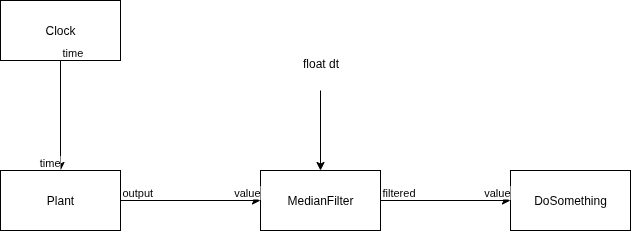
\includegraphics[width=\textwidth]{schema_median.png}
    \caption{Schéma du filtre médian}
    \label{fig:schema_median}
\end{figure}
%
\begin{figure}
    \centering
    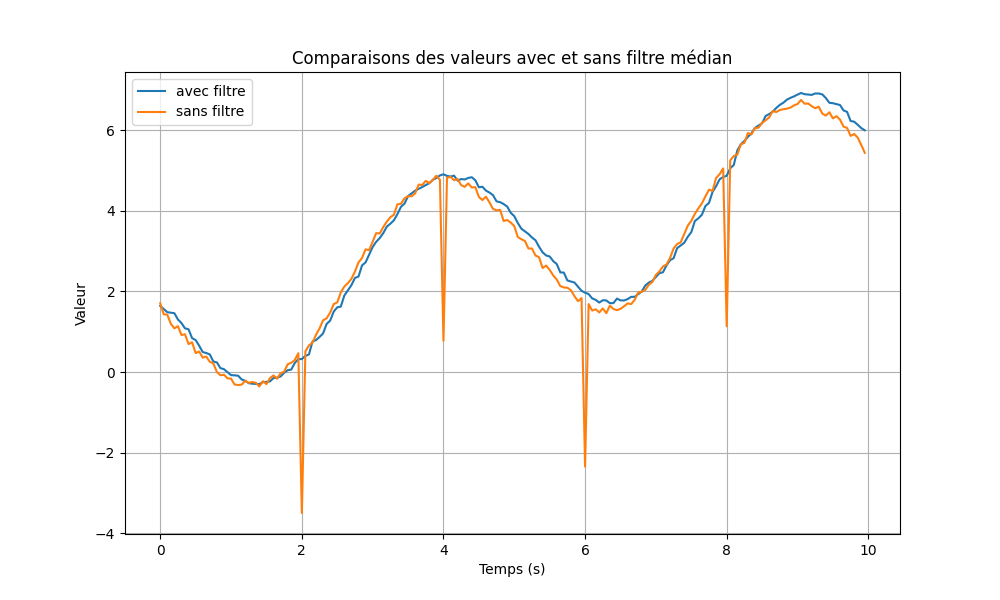
\includegraphics[width=\textwidth]{median.png}
    \caption{Résultat du filtre médian sur les données}
    \label{fig:median}
\end{figure}

\subsection{Anti-windup}

Maintenant j'utilise le même exemple (celui du drone) avec 2 anti-windup différents : le clamp et le back-calculation.
Pour permettre de comparer les 2 méthodes, j'ai utilisé les mêmes données pour les 2 méthodes.

Pour calculer l'altitude du drone en fonction du temps, j'utilise les équations suivantes :
$$K = 4 * k_p * (\frac{2\pi}{60})^{2}$$
$$F_p = K * \Omega_{rpm}^{2}$$
$$drag = DRAG\_COEFF * velocity$$
$$\alpha = \frac{F_p}{m} - g - (\frac{drag}{m})$$

Où : 
\begin{itemize}
    \item $k_p$ est la constante de poussée propre à chaque hélice, ici égale à 0.29
    \item $\Omega_{rpm}$ est la vitesse de rotation de l'hélice en tours par minute, qui correspond à la commande du contrôleur
    \item $DRAG\_COEFF$ est le coefficient de traînée, que j'ai choisi égal à 0.8
    \item $velocity$ est la vitesse du drone, que je calcule en intégrant l'accélération $\alpha$ au cours du temps
    \item $m$ est la masse du drone, que j'ai choisie égale à 0.2 kg
    \item $g$ est l'accélération due à la gravité, que j'ai choisie égale à 9.81 m/s²
\end{itemize}

L'objectif est de faire en sorte que le drone atteigne une altitude de 5 mètres et qu'on le garde au sol pendant 10 secondes et de voir comment les différentes méthodes d'anti-windup affectent la performance du système.

\subsubsection{Clamp}

L'anti-windup clamp consiste à limiter la valeur de l'intégral pour éviter qu'elle ne dépasse 2 certaines limites (maximal et minimal). Si l'intégral dépasse ces limites, il est "clampé" à la limite correspondante.
Ici la limite maximale est de 30 et la limite minimale est de -30.

L'observation flagrante est qu'au niveau de l'intégral (cf figure \ref{fig:integral_clamp}) on voit que l'intégral 
est clampé à 30 pendant une partie du temps, ce qui correspond à la période où le drone est au sol et que la 
commande est maximale pour essayer de faire décoller le drone.

\begin{figure}
    \centering
    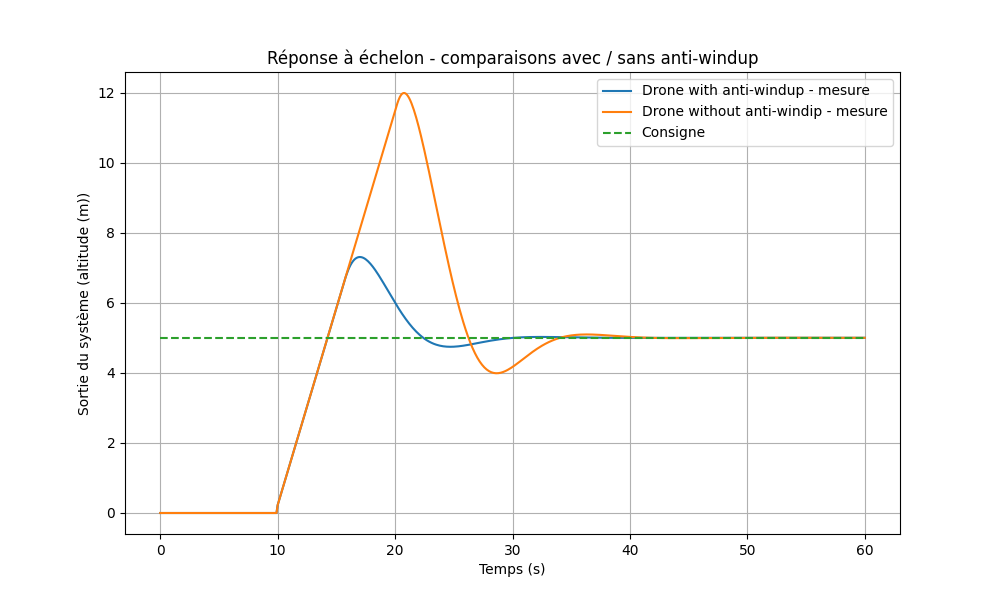
\includegraphics[width=\textwidth]{altitude_drone_clamp.png}
    \caption{Résultat de l'anti-windup sur les données}
    \label{fig:alt_clamp}
\end{figure}

\begin{figure}
    \centering
    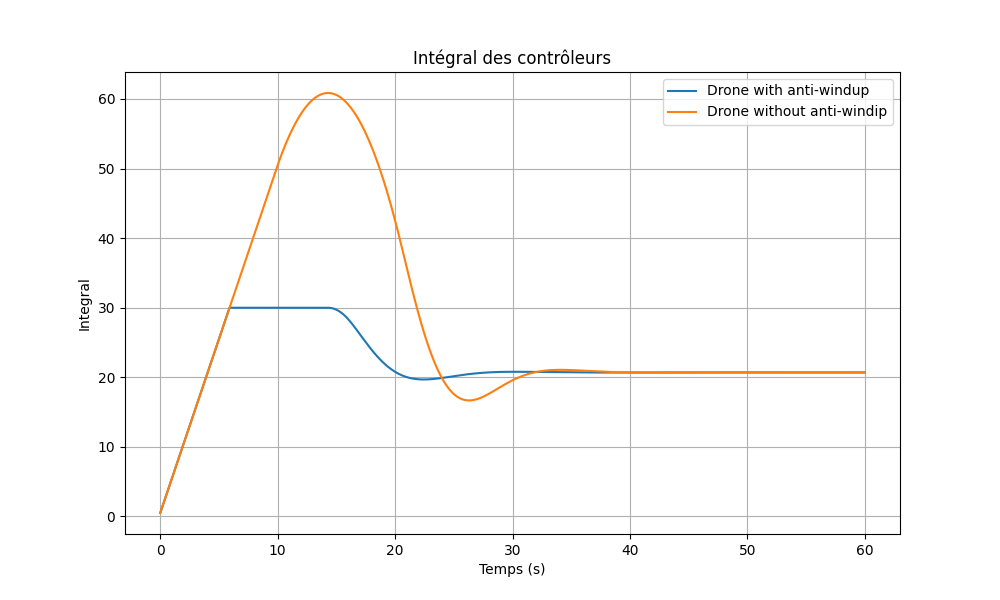
\includegraphics[width=\textwidth]{integral_drone_clamp.png}
    \caption{Intégral au cours du temps avec anti-windup}
    \label{fig:integral_clamp}
\end{figure}

\begin{figure}
    \centering
    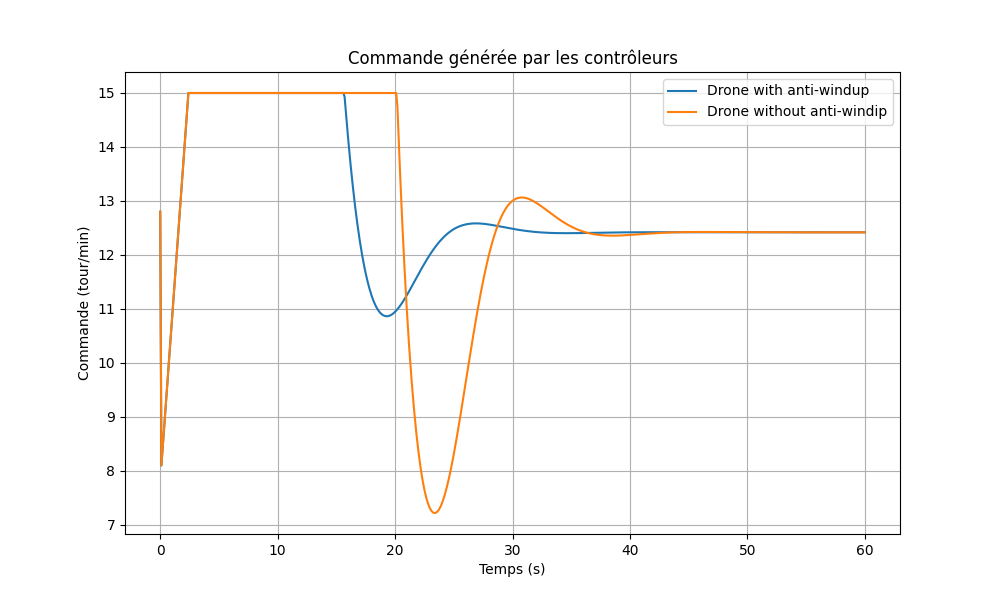
\includegraphics[width=\textwidth]{helice_drone_clamp.png}
    \caption{Résultat de l'anti-windup sur les données}
    \label{fig:blade_clamp}
\end{figure}

\subsubsection{Back-Calculation}

L'anti-windup back-calculation consiste à calculer une correction à appliquer à l'intégral en fonction de la différence entre la commande maximale et la commande réelle. Cette correction est ensuite soustraite de l'intégral pour éviter qu'il ne dépasse les limites.
Ici la correction est calculée en utilisant une constante de gain de back-calculation égale à 0.2.
La correction est calculée comme suit :
$$integral = integral + \frac{(satOutput - rawOutput)}{m\_Tt * dt}$$

où :
\begin{itemize}
    \item $satOutput$ est la commande maximale (ou minimale) à laquelle la sortie est limitée
    \item $rawOutput$ est la commande réelle calculée par le contrôleur
    \item $m\_Tt$ est la constante de gain de back-calculation, que j'ai choisie égale à 0.2
    \item $dt$ est le pas de temps entre les échantillons, que j'ai choisi égal à 0.1 secondes
\end{itemize}

\begin{figure}
    \centering
    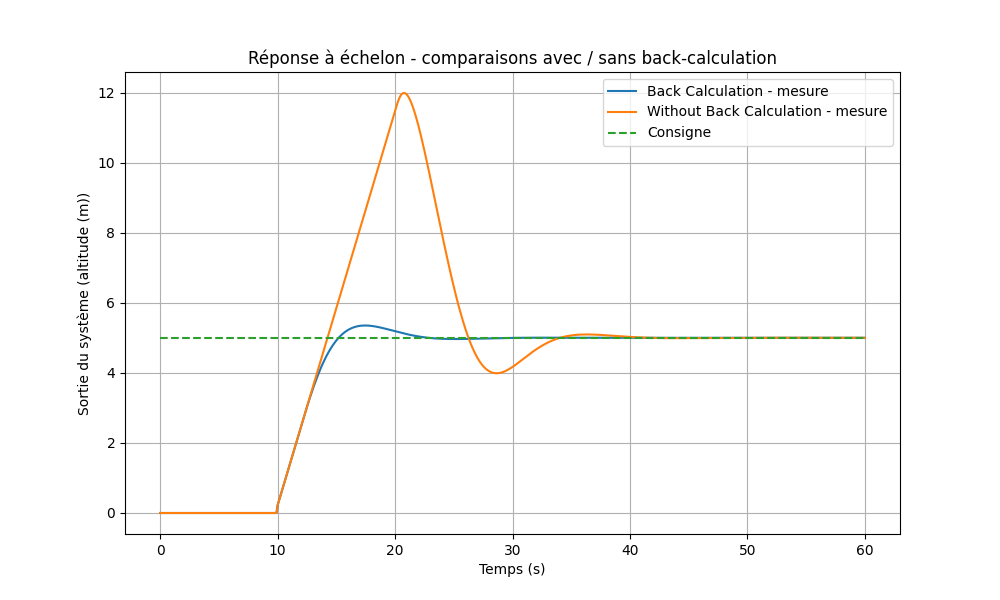
\includegraphics[width=\textwidth]{altitude_drone_backcalc.png}
    \caption{Résultat de l'anti-windup sur les données}
    \label{fig:alt_backcalc}
\end{figure}

\begin{figure}
    \centering
    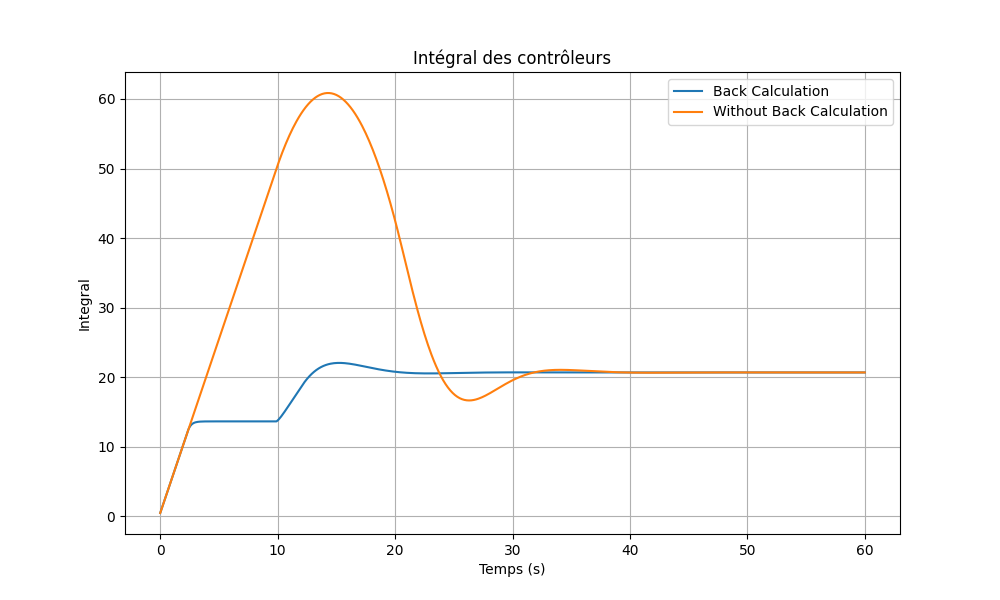
\includegraphics[width=\textwidth]{integral_drone_backcalc.png}
    \caption{Intégral au cours du temps avec anti-windup}
    \label{fig:integral_backcalc}
\end{figure}

\begin{figure}
    \centering
    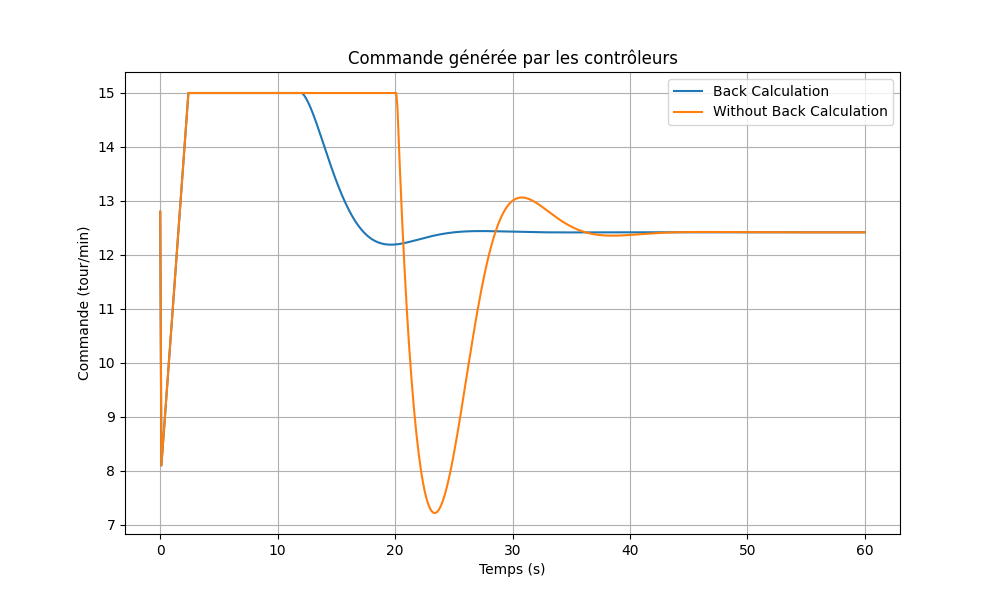
\includegraphics[width=\textwidth]{helice_drone_backcalc.png}
    \caption{Résultat de l'anti-windup sur les données}
    \label{fig:blade_backcalc}
\end{figure}

On peut se rendre compte que l'anti-windup back-calculation permet de réduire l'intégral de manière plus progressive que l'anti-windup clamp, ce qui peut permettre d'améliorer la performance du système en évitant les changements brusques de commande. (cf figure \ref{fig:integral_backcalc} et \ref{fig:integral_clamp})
De même pour la commande de l'hélice, on peut voir que l'anti-windup back-calculation permet d'avoir une commande plus fluide que l'anti-windup clamp, qui peut avoir des changements brusques de commande lorsque l'intégral est clampé. (cf figure \ref{fig:blade_backcalc} et \ref{fig:blade_clamp})
Et pour la montée en altitude, on peut voir que les 2 méthodes permettent au drone d'atteindre l'altitude cible de 5 mètres, mais que l'anti-windup back-calculation permet une montée plus fluide et moins brusque que l'anti-windup clamp. (cf figure \ref{fig:alt_backcalc} et \ref{fig:alt_clamp})

\section{Clarification interface chips}

J'ai clarifié l'interface chips pour les filtres et les anti-windup en créant une documentation détaillée qui explique comment utiliser ces outils dans différents systèmes.
J'ai également créé des diagrammes de blocs fonctionnels pour montrer comment les filtres et les anti-windup peuvent être intégrés dans différents systèmes de contrôle, ce qui peut aider à comprendre comment les utiliser de manière efficace.

\subsection{Filtres}

Ici, on va montrer avec un filtre passe-bas mais cela revient à la même chose pour les autres filtres.

Le diagramme de bloc fonctionnel pour le filtre passe-bas est le suivant (cf figure \ref{fig:schema_lowpass}) et le
programme chips correspondant est le suivant :
\begin{verbatim}
logical Clock() init {
	float dt = 0;
}then{
	dt = dt + 0.1;
} -> time(dt);

logical GenerateSample(float time) 
-> output(// Some value )

logical DoSomething(float value) then{
	// Do something
}

system{
	LowPassFilter lp;
	GenerateSample sample;
	Clock clock;
	DoSomething dostg;
	float dt = 0.1;
	float tau = // Some value
	sample.time(clock.time);
    lp{dt: dt, tau: tau, value: sample.output};
	dostg.value(lp.filtered);
}
\end{verbatim}

On pourrait lui associer une documentation qui explique comment utiliser le filtre (comme man pour les commandes bash) et qui ressemblerait à cela :
\begin{Verbatim}[breaklines=true]
LowPassFilter - A low-pass filter that allows low frequencies to pass through while attenuating high frequencies.
Usage:
    LowPassFilter{dt: <float>, tau: <float>, value: <float>}
Parameters:
    dt: The time step between samples, which determines how often the filter is updated.
    tau: The time constant of the filter, which determines how quickly the filter responds to changes in the input signal.
    value: The input signal to be filtered, which is a float value that can be generated by any logical block in the system.
Output:
    filtered: The filtered output signal, which is a float value that can be used by any logical block in the system.
Description:
    The LowPassFilter takes an input signal and applies a low-pass filter to it, allowing low frequencies to pass 
    through while attenuating high frequencies. The filter is updated at each time step defined by the dt parameter, 
    and the response of the filter is determined by the tau parameter. The filtered output can be used in any part 
    of the system, making it a versatile tool for signal processing in various applications.
\end{Verbatim}

\subsection{Anti-windup}

Pour l'anti-windup, on pourrait faire la même chose que pour les filtres en créant un diagramme de bloc fonctionnel pour chaque méthode d'anti-windup 
et en créant une documentation détaillée pour expliquer comment les utiliser dans différents systèmes de contrôle.

Le problème que je rencontre pour faire cela, c'est que l'anti-windup est directement intégré dans le contrôleur, ce qui rend difficile de l'utiliser 
de manière indépendante dans différents systèmes.
Car chaque anti-windup a des paramètres spécifiques qui permettent de l'adapter à différents systèmes de contrôle. 
La figure \ref{fig:idee_AW} montre une idée qui sera expliquée plus en détails lors de la réunion.

\begin{figure}
    \centering
    \includegraphics[width=\textwidth]{AW.jpg}
    \caption{Idée pour l'antiw-windup en CHIPS}
    \label{fig:idee_AW}
\end{figure}

\section{Plan rapport}

Pour le rapport de stage, je vais suivre le plan suivant :

\begin{enumerate}
    \item Introduction
    \item Présentation FEMTO-ST
    \item Littérature, contexte et objectifs $\rightarrow$ pour expliquer les différentes lectures que j'ai pu faire
    durant le stage et comment elles m'ont permis de mieux comprendre les différents concepts et les mettre en lien 
    avec les travaux que j'ai pu faire. Puis expliquer les objectifs du stage.
    \item Parseur/XMI $\rightarrow$ expliquer comment a été finalisé le parseur et comment il fonctionne, avec des exemples d'utilisation. De même pour la sérialisation vers XMI.
    \item Outils de la théorie de contrôle $\rightarrow$ Expliquer les différents outils qui ont pu être développés (filtres/anti-windups) et comment ils fonctionnent, avec des exemples d'utilisation. Expliquer comment ils peuvent être utilisés dans différents systèmes de contrôle.
    \item Conclusion et perspectives
\end{enumerate}

Le design pattern et les motifs de contrôle ne sont pas dans le plan car ils ne sont pas encore finalisés ou commencés, mais ils pourraient être ajoutés dans la section "Outils de la théorie de contrôle" ou dans une section séparée si nécessaire.


\end{document}